\documentclass[
11pt, % The default document font size, options: 10pt, 11pt, 12pt
codirector, % Uncomment to add a codirector to the title page
]{charter} 




% El títulos de la memoria, se usa en la carátula y se puede usar el cualquier lugar del documento con el comando \ttitle
\titulo{Placa de prueba para block de energía} 

% Nombre del posgrado, se usa en la carátula y se puede usar el cualquier lugar del documento con el comando \degreename
\posgrado{Carrera de Especialización en Sistemas Embebidos} 
%\posgrado{Carrera de Especialización en Internet de las Cosas} 
%\posgrado{Carrera de Especialización en Intelegencia Artificial}
%\posgrado{Maestría en Sistemas Embebidos} 
%\posgrado{Maestría en Internet de las cosas}

% Tu nombre, se puede usar el cualquier lugar del documento con el comando \authorname
\autor{Marcos Raul Dominguez Shocron} 

% El nombre del director y co-director, se puede usar el cualquier lugar del documento con el comando \supname y \cosupname y \pertesupname y \pertecosupname
\director{Yaki Nachajon Schwartz}
\pertenenciaDirector{FIUBA} 
% FIXME:NO IMPLEMENTADO EL CODIRECTOR ni su pertenencia
\codirector{John Doe} % para que aparezca en la portada se debe descomentar la opción codirector en el documentclass
\pertenenciaCoDirector{FIUBA}

% Nombre del cliente, quien va a aprobar los resultados del proyecto, se puede usar con el comando \clientename y \empclientename
\cliente{Gillermo Gebhart}
\empresaCliente{Voltu Motors}

% Nombre y pertenencia de los jurados, se pueden usar el cualquier lugar del documento con el comando \jurunoname, \jurdosname y \jurtresname y \perteunoname, \pertedosname y \pertetresname.
\juradoUno{Nombre y Apellido (1)}
\pertenenciaJurUno{pertenencia (1)} 
\juradoDos{Nombre y Apellido (2)}
\pertenenciaJurDos{pertenencia (2)}
\juradoTres{Nombre y Apellido (3)}
\pertenenciaJurTres{pertenencia (3)}
 
\fechaINICIO{24 de junio de 2021}		%Fecha de inicio de la cursada de GdP \fechaInicioName
\fechaFINALPlan{19 de agosto de 2021} 	%Fecha de final de cursada de GdP
\fechaFINALTrabajo{15 de mayo de 2022}	%Fecha de defensa pública del trabajo final


\begin{document}

\maketitle
\thispagestyle{empty}
\pagebreak


\thispagestyle{empty}
{\setlength{\parskip}{0pt}
	\tableofcontents{}
}
\pagebreak


\section*{Registros de cambios}
\label{sec:registro}


\begin{table}[ht]
	\label{tab:registro}
	\centering
	\begin{tabularx}{\linewidth}{@{}|c|X|c|@{}}
		\hline
		\rowcolor[HTML]{C0C0C0}
		Revisión & \multicolumn{1}{c|}{\cellcolor[HTML]{C0C0C0}Detalles de los cambios realizados} & Fecha            \\ \hline
		0        & Creación del documento                                                          & \fechaInicioName \\ \hline
		1        & Se completa hasta el punto 5 inclusive                                          & 6 de julio 2021  \\ \hline
		2        & Se completa hasta el punto 9 inclusive                                          & 13 de julio 2021 \\ \hline
		3        & Se completa hasta el punto 11 inclusive                                         & 27 de julio 2021 \\ \hline
		3.1      & Se completa hasta el punto 12 inclusive                                         & 31 de julio 2021 \\ \hline
		4        & Se completa el plan                                                             & 5 de agosto 2021 \\ \hline
	\end{tabularx}
\end{table}

\pagebreak



\section*{Acta de constitución del proyecto}
\label{sec:acta}

\begin{flushright}
	Buenos Aires, \fechaInicioName
\end{flushright}

\vspace{2cm}

Por medio de la presente se acuerda con el Ing. \authorname\hspace{1px} que su Trabajo Final de la \degreename\hspace{1px} se titulará ``\ttitle'',
consistirá esencialmente en una placa de prueba para validar los desarrollos de la placa de control del block de energía, y
tendrá un presupuesto preliminar estimado de 610 hs de trabajo y \$1275000, con fecha de inicio \fechaInicioName\hspace{1px} y
fecha de presentación pública \fechaFinalName.

Se adjunta a esta acta la planificación inicial.

\vfill

% Esta parte se construye sola con la información que hayan cargado en el preámbulo del documento y no debe modificarla
\begin{table}[ht]
	\centering
	\begin{tabular}{ccc}
		\begin{tabular}[c]{@{}c@{}}Ariel Lutenberg \\ Director posgrado FIUBA\end{tabular} & \hspace{2cm} & \begin{tabular}[c]{@{}c@{}}\clientename \\ \empclientename \end{tabular} \vspace{2.5cm} \\
		\multicolumn{3}{c}{\begin{tabular}[c]{@{}c@{}} \supname \\ Director del Trabajo Final\end{tabular}} \vspace{2.5cm}                        \\
		%\begin{tabular}[c]{@{}c@{}}\jurunoname \\ Jurado del Trabajo Final\end{tabular}     &  & \begin{tabular}[c]{@{}c@{}}\jurdosname\\ Jurado del Trabajo Final\end{tabular}  \vspace{2.5cm}  \\
		%\multicolumn{3}{c}{\begin{tabular}[c]{@{}c@{}} \jurtresname\\ Jurado del Trabajo Final\end{tabular}} \vspace{.5cm}                                                                     
	\end{tabular}
\end{table}




\section{1. Descripción técnica-conceptual del proyecto a realizar}
\label{sec:descripcion}


Un block de energía es un dispositivo de almacenamiento y gestión de energía que se crea como una alternativa a los grupos electrógenos. Estos dispositivos almacenan energía en baterías con autonomías superiores a los 7 [KWh] y la suministran cuando es necesario. Típicamente entregan la tensión de red cuando se corta el suministro principal de energía eléctrica.

Para cumplir su función este dispositivo mide distintas señales del entorno y utiliza estos datos para tomar decisiones. Actualmente es muy complejo generar las condiciones de entorno para verificar que el equipo desarrollado reacciona según lo esperado.
El sistema embebido a desarrollar debe generar las posibles señales, que el bloque de energía sensa, para corroborar que el equipo responde adecuadamente ante las posibles situaciones del entorno.

El sistema actual reporta su estado general, las fallas y el estado de sus periféricos. Estos reportes se pueden utilizar para evaluar el comportamiento del equipo. Se espera que generando las señales que el equipo mide para tomar decisiones se pueda evaluar su respuesta.

En la Figura \ref{fig:diagBloques} se puede observar cómo se integra la propuesta de sistema embebido con el block de energía. Adicionalmente se pueden observar las señales que se pretenden generar. Las señales enlistadas permiten tomar la mayoría de las decisiones al sistema de control.

El sistema de control también toma decisiones en función de la información que recibe del sistema de gestión de batería (en inglés, Battery Management System, BMS). El proyecto actual no simulará la comunicación del BMS. Esto impacta sobre los ensayos y la forma de utilizar la placa de prueba. Para que el BMS no interfiera en las pruebas con la placa a desarrollar, se deberá contar con una batería en buenas condiciones.

Un dispositivo de estas características permite a los desarrolladores validar un cambio en el firmware, o una nueva funcionalidad, con sencillez y velocidad.

%\vspace{25px}

\begin{figure}[htpb]
	\centering
	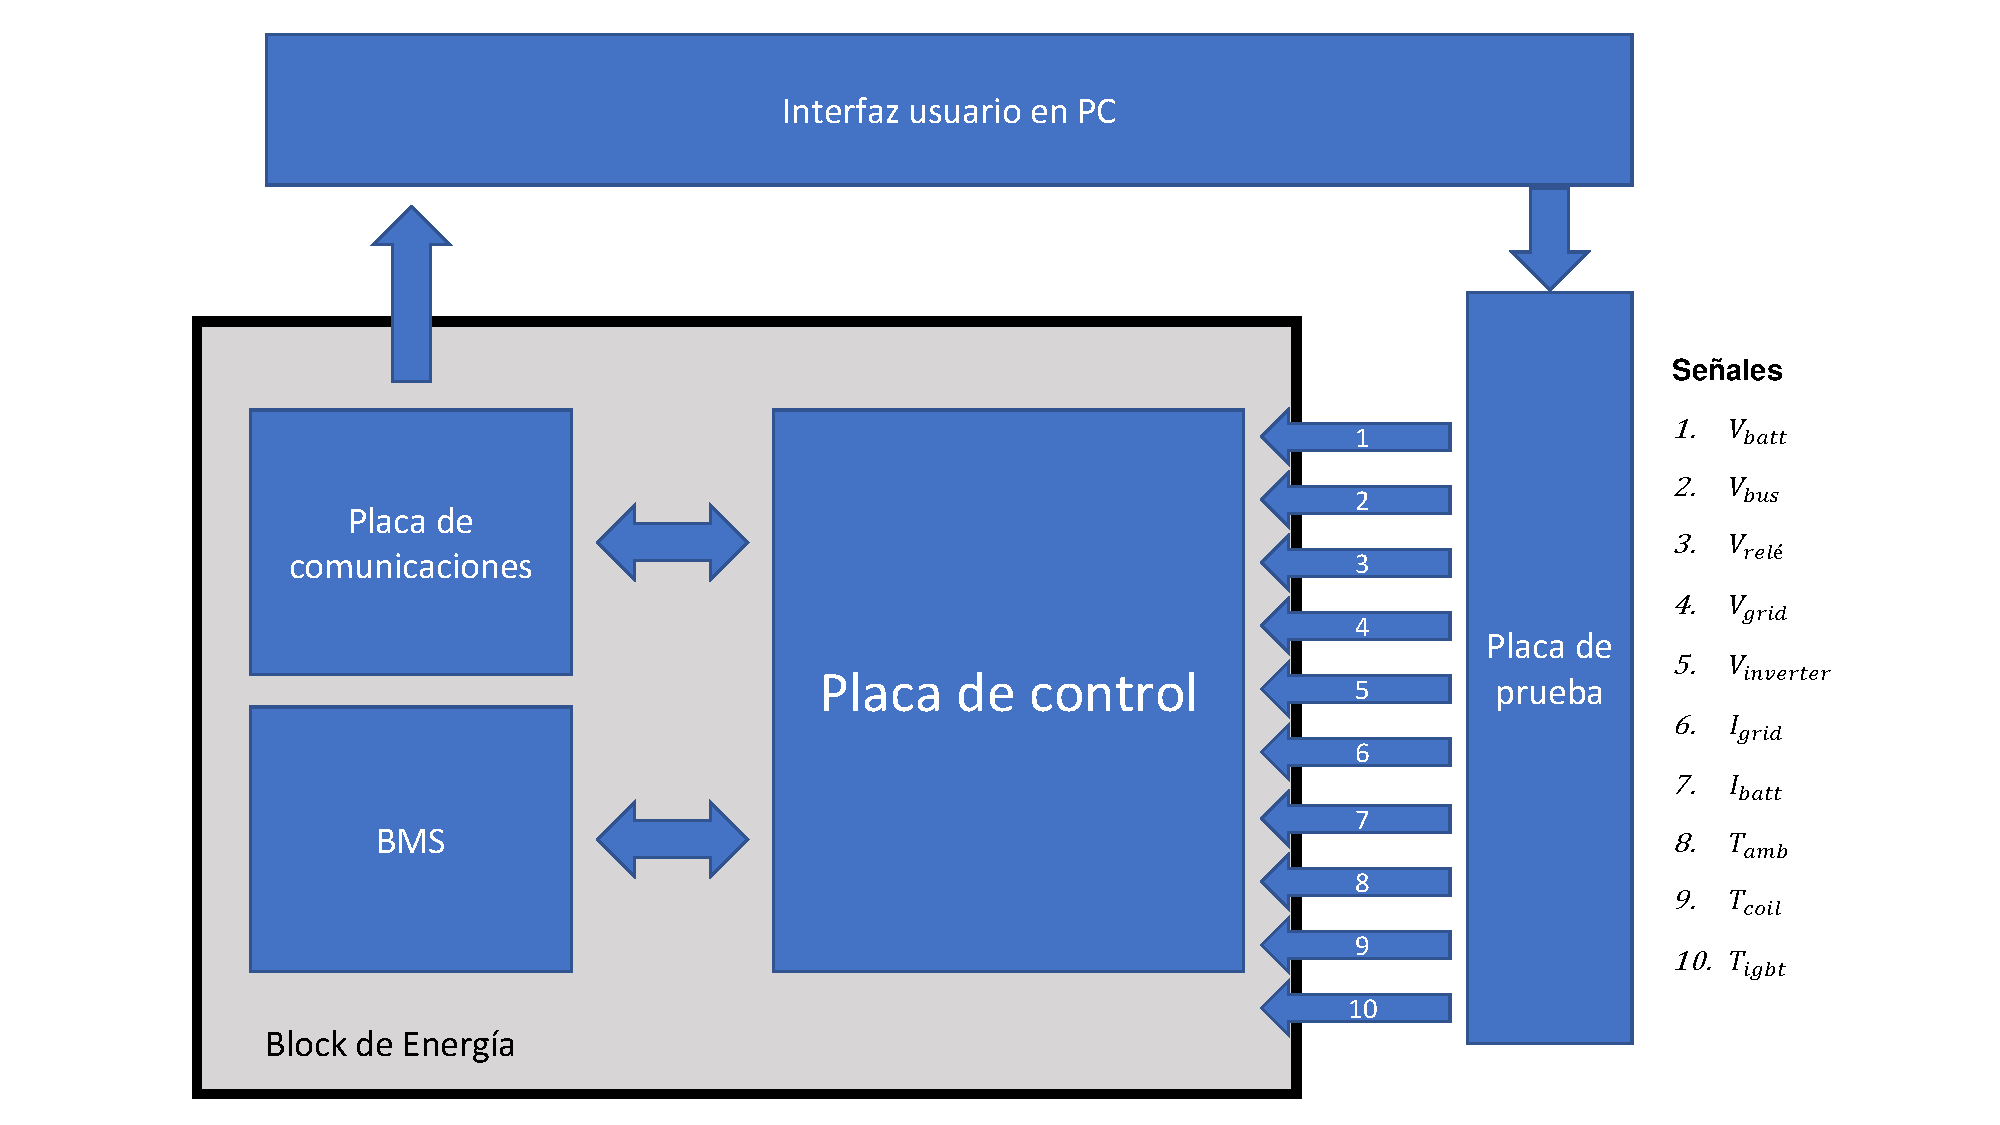
\includegraphics[width=1\textwidth]{./Figuras/DiagramaEnBloqueDelProyecto.pdf}
	\caption{Diagrama en bloques del sistema.}
	\label{fig:diagBloques}
\end{figure}

\vspace{25px}

Como se introdujo anteriormente, se generarán una serie de señales que permitan simular las condiciones de entorno que mide la placa de control.
Este desarrollo permitirá entonces verificar si la placa de control responde adecuadamente a las reglas establecidas.

Como se representa en la Figura \ref{fig:diagBloques}, se generarán diez señales para realizar las pruebas. Las señales de tensión son efectivamente tensiones no escaladas, por lo que tienen valores de 220 V en alterna o alrededor de 400 V continua.

Las señales de corrientes son medidas por un transductor que convierte el valor medido en tensión, por lo que el valor de señal a inyectar a la placa es una tensión en el rango de los 0 a 5 V. Este rango simula una corriente de -50 a 50 A.

Finalmente las temperaturas se miden con NTC, por lo que las señales 8, 9 y 10 deben ser en Ohms. Esto se realizará con el uso de potenciómetros digitales que cambian su valor para simular los cambios de temperatura.

La placa de prueba será comandada por medio de una interfaz por computadora. En la primera versión el usuario podrá establecer las señales para generar y evaluar el comportamiento del equipo.

Para lograr las señales de tensión el equipo deberá estar conectado a una alimentación de red, a una batería igual a la del equipo cargada y alimentada por el USB de comunicación.
Este proyecto se vincula con el proceso de desarrollo del block de energía de la empresa Voltu y será utilizado para testear los avances de desarrollo del equipo. Se espera también que permita realizar el control de los equipos en la etapa de producción.



\section{2. Identificación y análisis de los interesados}
\label{sec:interesados}

\begin{table}[ht]
	%\caption{Identificación de los interesados}
	%\label{tab:interesados}
	\begin{tabularx}{\linewidth}{@{}|l|X|X|l|@{}}
		\hline
		\rowcolor[HTML]{C0C0C0}
		Rol           & Nombre y Apellido & Organización    & Puesto                 \\ \hline
		Cliente       & \clientename      & \empclientename & CEO                    \\ \hline
		Impulsor      & \clientename      & \empclientename & CEO                    \\ \hline
		Responsable   & \authorname       & FIUBA           & Alumno                 \\ \hline
		Orientador    & \supname          & \pertesupname   & Director Trabajo final \\ \hline
		Usuario final & Carlos Zalayeta   & \empclientename & Desarrollador          \\ \hline
	\end{tabularx}
\end{table}



\section{3. Propósito del proyecto}
\label{sec:proposito}

El propósito de este proyecto es desarrollar un dispositivo que permita evaluar, de forma parcial, el comportamiento de la placa de control del block de energía durante su desarrollo.


\section{4. Alcance del proyecto}
\label{sec:alcance}
A  se detalla el alcance del proyecto y sus limitaciones.
\begin{itemize}
	\item Alcances
	      \begin{itemize}
		      \item Se realizará un prototipo que permita generar las 10 señales listadas en la Figura \ref{fig:diagBloques}.
		      \item Se desarrollará un prototipo que permita configurar los valores de las señales en tiempo real.
	      \end{itemize}
	\item Limitaciones
	      \begin{itemize}
		      \item No se simulará la comunicación con el BMS.
		      \item No se analizará el comportamiento del equipo por software.
		      \item Se desarrollará un prototipo sin embalaje y sin chasis.
		      \item Solo dispondrá la electrónica y conectores necesarios.
	      \end{itemize}
\end{itemize}


\section{5. Supuestos del proyecto}
\label{sec:supuestos}

Para el desarrollo del presente proyecto se supone que:
\begin{itemize}
	\item Se dispondrá de al menos una placa de control funcional durante todo el desarrollo.
	\item Se dispondrá de al menos una placa de comunicación funcional durante todo el desarrollo.
	\item Se dispondrá de al menos una batería con su BMS completo y funcional durante todo el desarrollo.
	\item Se dispondrá de señales estables de tensión alterna para el uso del sistema.
	\item Se dispondrá de acceso a los interesados de forma regular para discutir los avances.

\end{itemize}


\section{6. Requerimientos}
\label{sec:requerimientos}

\begin{enumerate}
	\item Interfases
	      \begin{enumerate}
		      \item El sistema debe poder comunicarse con una PC
		      \item El sistema debe poseer un botón de encendido
		      \item El sistema debe tener actuadores que simulen una señal de potencia.
		      \item El sistema debe tener actuadores con señales de baja tensión.
		      \item El sistema debe tener actuadores resistivos.
		      \item El sistema debe informar el estado de las señales (on/off).
	      \end{enumerate}
	\item Requerimientos funcionales
	      \begin{enumerate}
		      \item Emulación de altas tensiones continuas
		            \begin{enumerate}
			            \item El sistema debe controlar salidas de tensión que emulen las tensiones de continua elevadas que mide el block de energía.
			            \item El sistema debe permitir que el usuario configure el valor de tensión continua elevada a emular.
			            \item El sistema debe reportar error si no se configura un valor válido de tensión.
			            \item El sistema debe permitir configurar las tensiones elevadas continuas Vbatt, Vbus y Vrelé de la Figura 1 de forma independiente.
			            \item El sistema emulará tensiones de bus, batería y relé en un rango comprendido entre 0 V a 450 V.
		            \end{enumerate}
		      \item Simulación de corriente con bajas tensiones de continua
		            \begin{enumerate}
			            \item El sistema debe controlar salidas de tensión que simulen la medición de corriente de los sensores utilizados por el block de energía.
			            \item El sistema debe permitir que el usuario configure el valor de corriente a simular.
			            \item El sistema debe reportar error si no se configura un valor válido de corriente.
			            \item El sistema debe permitir configurar las corrientes Igrid e Ibatt de la Figura \ref{fig:diagBloques} de forma independiente.
			            \item El sistema simulará corrientes desde 0 A a 50 A.
		            \end{enumerate}
		      \item Emulación de tensiones alternas
		            \begin{enumerate}
			            \item El sistema debe controlar salidas de tensión que emulen las tensiones alternas que mide el block de energía.
			            \item El sistema debe permitir que el usuario configure el valor de tensión a emular.
			            \item El sistema debe reportar error si no se configura un valor válido de tensión alterna.
			            \item El sistema debe permitir configurar las tensiones alternas Vgrid y Vinverter de la Figura \ref{fig:diagBloques} de forma independiente.
			            \item El sistema emulará tensiones alternas (Vinverter y Vgrid) en un rango comprendido entre 0 y 240 Vrms.
		            \end{enumerate}
		      \item Simulación de temperaturas
		            \begin{enumerate}
			            \item El sistema debe controlar resistencias variables que emulen la variación de resistencia de un termistor NTC por temperatura.
			            \item El sistema debe permitir que el usuario configure el valor de temperatura a emular.
			            \item El sistema debe reportar error si no se configura un valor válido de temperatura.
			            \item El sistema debe permitir configurar las temperaturas Tcoil, Tigbt y ambiente de la Figura \ref{fig:diagBloques} de forma independiente.
			            \item El sistema simulará las temperaturas en un rango comprendido entre 5 a 150 ºC.
		            \end{enumerate}
	      \end{enumerate}
	\item Requerimientos de rendimiento
	      \begin{enumerate}
		      \item El sistema debe actuar en un tiempo menor a 150 ms luego de recibir un comando del usuario.
	      \end{enumerate}
\end{enumerate}

\section{7. Historias de usuarios (\textit{Product backlog})}
\label{sec:backlog}

En esta sección se incluyen las historias de usuarios y su ponderación (\textit{story points}).

``Como desarrollador quiero poder suministrar distintos valores de tensión de linea al control para validar la generación."

Dificultad: alta (5) - Implica muchas horas de diseño de hardware y software.

Complejidad: alta (5) - Realizar un diseño seguro cuando se manejan valores de tensión elevados requiere de un cuidando superior.

Riesgo: alta (5) - Durante los ensayos de esta funcionalidad es probable que se quemen componentes y existe el riesgo de electrochoque.

\textit{story points}: 13
(5 + 5 + 3 = 15 -- 13 es el valor más cercano en Fibonacci)

``Como desarrollador quiero poder suministrar distintos valores de tensión de a la medición de batería al control para validar la entrada y salida del modo carga."

Dificultad: alta (5) - Implica muchas horas de diseño de hardware y software.

Complejidad: alta (5) - Realizar un diseño seguro cuando se manejan valores de tensión elevados requiere de un cuidando superior.

Riesgo: alta (5) - Durante los ensayos de esta funcionalidad es probable que se quemen componentes y existe el riesgo de electrochoque.

\textit{story points}: 13
(5 + 5 + 3 = 15 -- 13 es el valor más cercano en Fibonacci)

``Como desarrollador quiero poder variar los valores de resistencia medidos por la placa de control para validar el encendido/apagado de los circuitos de refrigeración.

Dificultad: alta (5) - Implica muchas horas de diseño de hardware y software.

Complejidad: baja (1) - El manejo de potenciómetros digitales para variar resistencia no supone un nivel elevado de complejidad.

Riesgo: bajo (1) - La variación de potenciómetros digitales alimentados a 5 V no suponen un riesgo elevado.

\textit{story points}: 8
(5 + 1 + 1 = 7 -- 8 es el valor más cercano en Fibonacci)

``Como desarrollador quiero poder simular las corrientes medidas por la placa de control para validar las protecciones del sistema de control.

Dificultad: alta (5) - Implica muchas horas de diseño de hardware y software.

Complejidad: baja (1) - El manejo de tensiones analógicas bajas para simular salidas de sensores de corrientes no requiere de un \textit{know-how} muy específico y difícil de conseguir.

Riesgo: bajo (1) - El uso de bajas tensiones no produce grandes riesgos en su manipulación.

\textit{story points}: 8
(5 + 1 + 1 = 7 -- 8 es el valor más cercano en Fibonacci)

``Como desarrollador quiero poder enviar comandos por una terminal desde la PC para configurar las señales que se enviarán desde la placa de prueba.

Dificultad: alta (5) - Implica muchas horas de diseño de hardware y software.

Complejidad: media (3) - El diseño e implementación del protocolo de comunicación y la interfaz tienen una complejidad elevada.

Riesgo: bajo (1) - No existen grandes riesgos en el desarrollo de una interfaz de comunicación con la placa de prueba.

\textit{story points}: 8
(5 + 3 + 1 = 9 -- 8 es el valor más cercano en Fibonacci)

\section{8. Entregables principales del proyecto}
\label{sec:entregables}

\begin{itemize}
	\item Manual de uso
	\item Diagrama de circuitos esquemáticos
	\item Código fuente del firmware
	\item Diagrama de instalación
	\item Informe final
	\item Prototipo
\end{itemize}

\section{9. Desglose del trabajo en tareas}
\label{sec:wbs}

\begin{enumerate}
	\item Hardware
	      \begin{enumerate}
		      \item Decidir micro a utilizar (40 hs).
		      \item Decidir reguladores de tensión alterna (20 hs).
		      \item Diseñar salidas analógicas de baja tensión (20 hs).
		      \item Elegir método para simular NTC (20 hs).
		      \item Diseñar integralmente el hardware (40 hs).
		      \item Solicitar el primer prototipo (5 hs).
	      \end{enumerate}
	\item Firmware
	      \begin{enumerate}
		      \item Crear repositorio (0.5 hs).
		      \item Diseñar las maquinas de estado (40 hs).
		      \item Implementar el protocolo de comunicación con PC (40 hs).
		      \item Implementar simulación de señales de corriente (40 hs).
		      \item Implementar emulación de señales de tensón alterna (40 hs).
		      \item Implementar emulación de señales de tensión continua (40 hs).
		      \item Implementar simulación de señales de temperatura (40 hs).
	      \end{enumerate}
	\item Validación
	      \begin{enumerate}
		      \item Validar las temperaturas simuladas (5 hs).
		      \item Validar las corrientes simuladas	(5 hs).
		      \item Validar las tensiones continuas simuladas (5 hs).
		      \item Validar las tensiones alternas simuladas (5 hs).
		      \item Validar el funcionamiento integral con un block de energía (20 hs).
	      \end{enumerate}
	\item Informe de avances
	      \begin{enumerate}
		      \item Redacción de avances en el diseño del Hardware (8 hs).
		      \item Redacción de avances en el diseño del Firmware (8 hs).
		      \item Redacción de avances en la validación del sistema (8 hs).
	      \end{enumerate}
	\item Memoria
	      \begin{enumerate}
		      \item Redacción del marco teórico (40 hs).
		      \item Redacción del diseño y arquitectura del Hardware (40 hs).
		      \item Redacción del diseño y arquitectura del firmware (40 hs).
		      \item Formulación de conclusiones (20 hs).
		      \item Corrección del documento (20 hs).
	      \end{enumerate}
\end{enumerate}

Cantidad total de horas: 609.5 hs.
\begin{landscape}
	\section{10. Diagrama de Activity On Node}
	\label{sec:AoN}

	\begin{figure}[htpb]
		\centering
		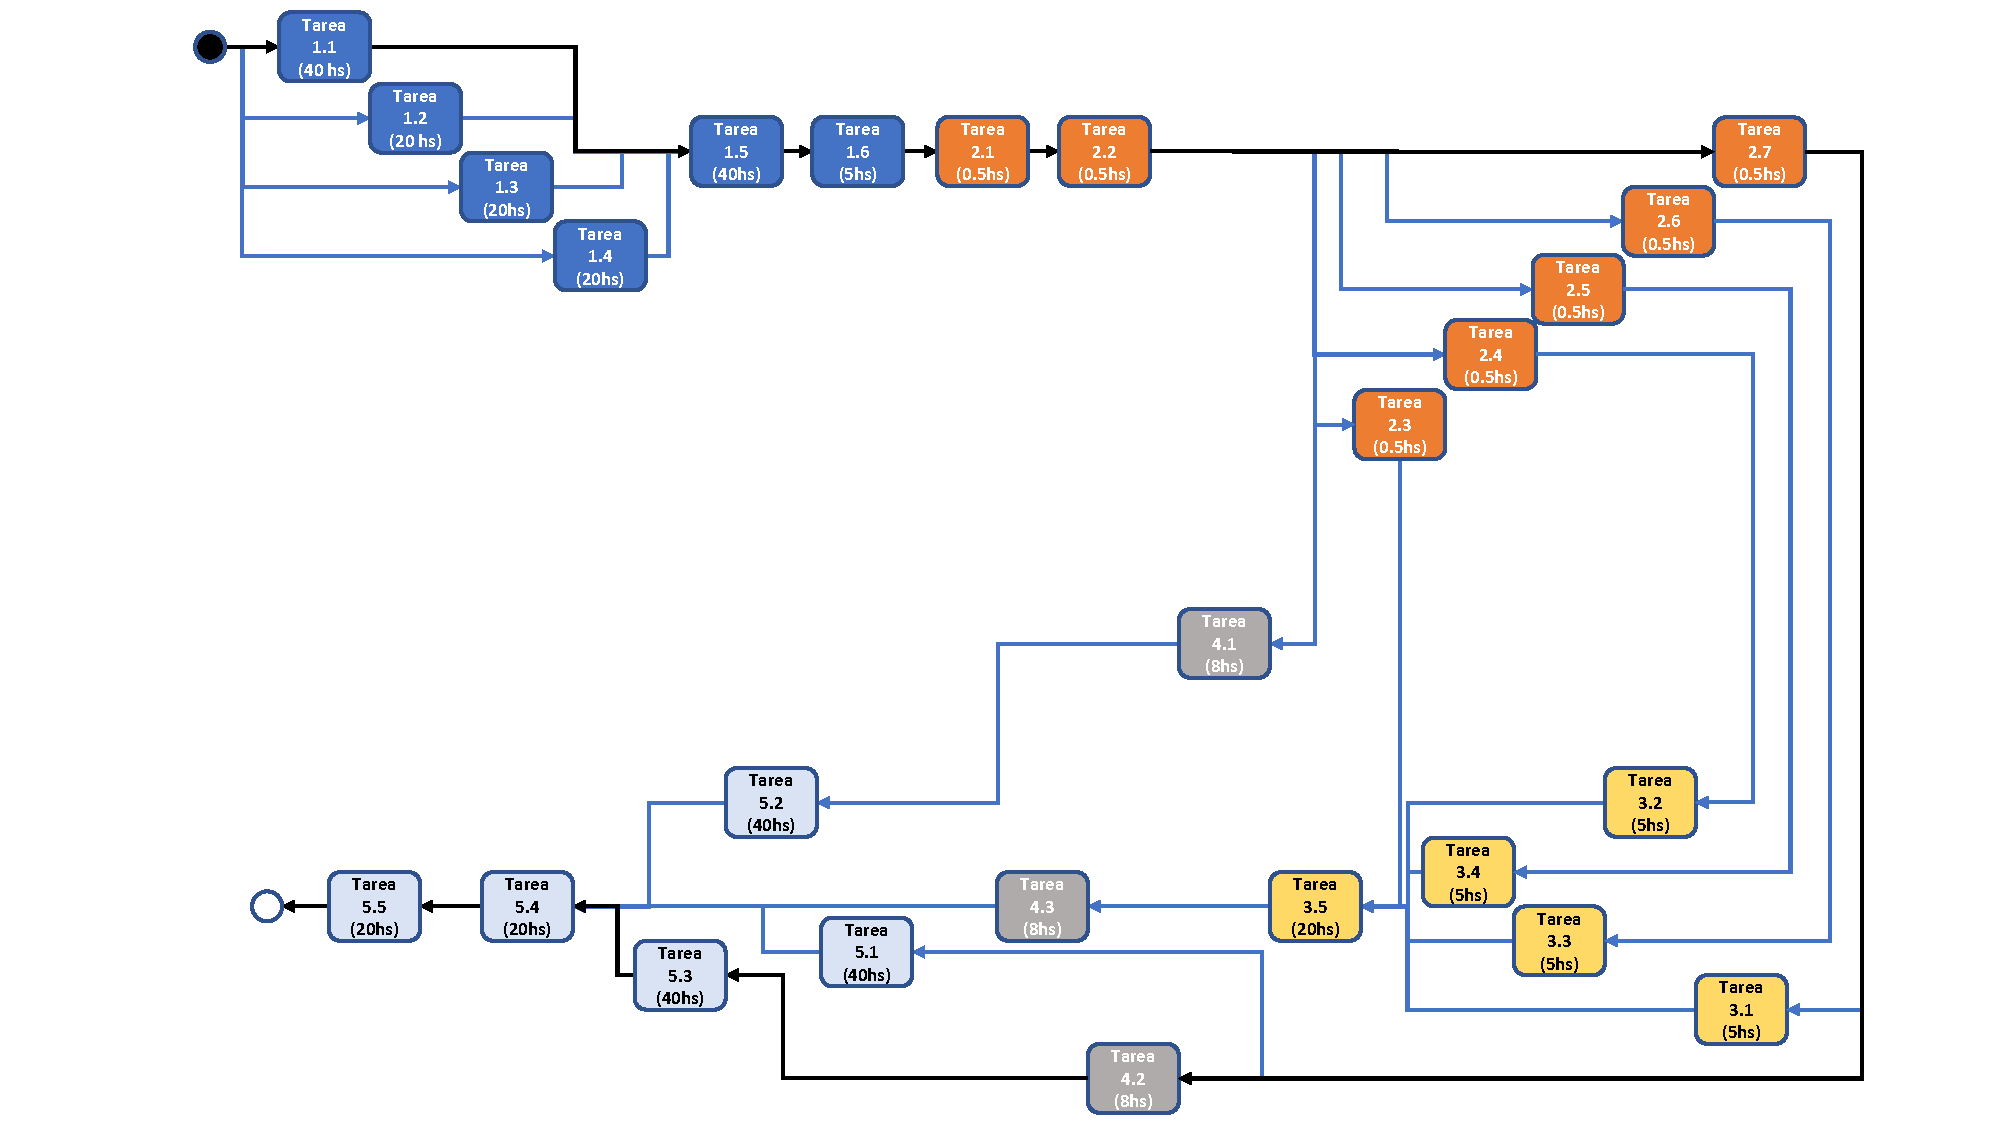
\includegraphics[width=1.5\textwidth]{./Figuras/Aon_cropped.pdf}
		\caption{Diagrama en \textit{Activity on Node}}
		\label{fig:AoN}
	\end{figure}
\end{landscape}

\begin{landscape}
	\label{sec:gantt}
	\section{11. Diagrama de Gantt}
	\begin{figure}[htpb]
		\centering
		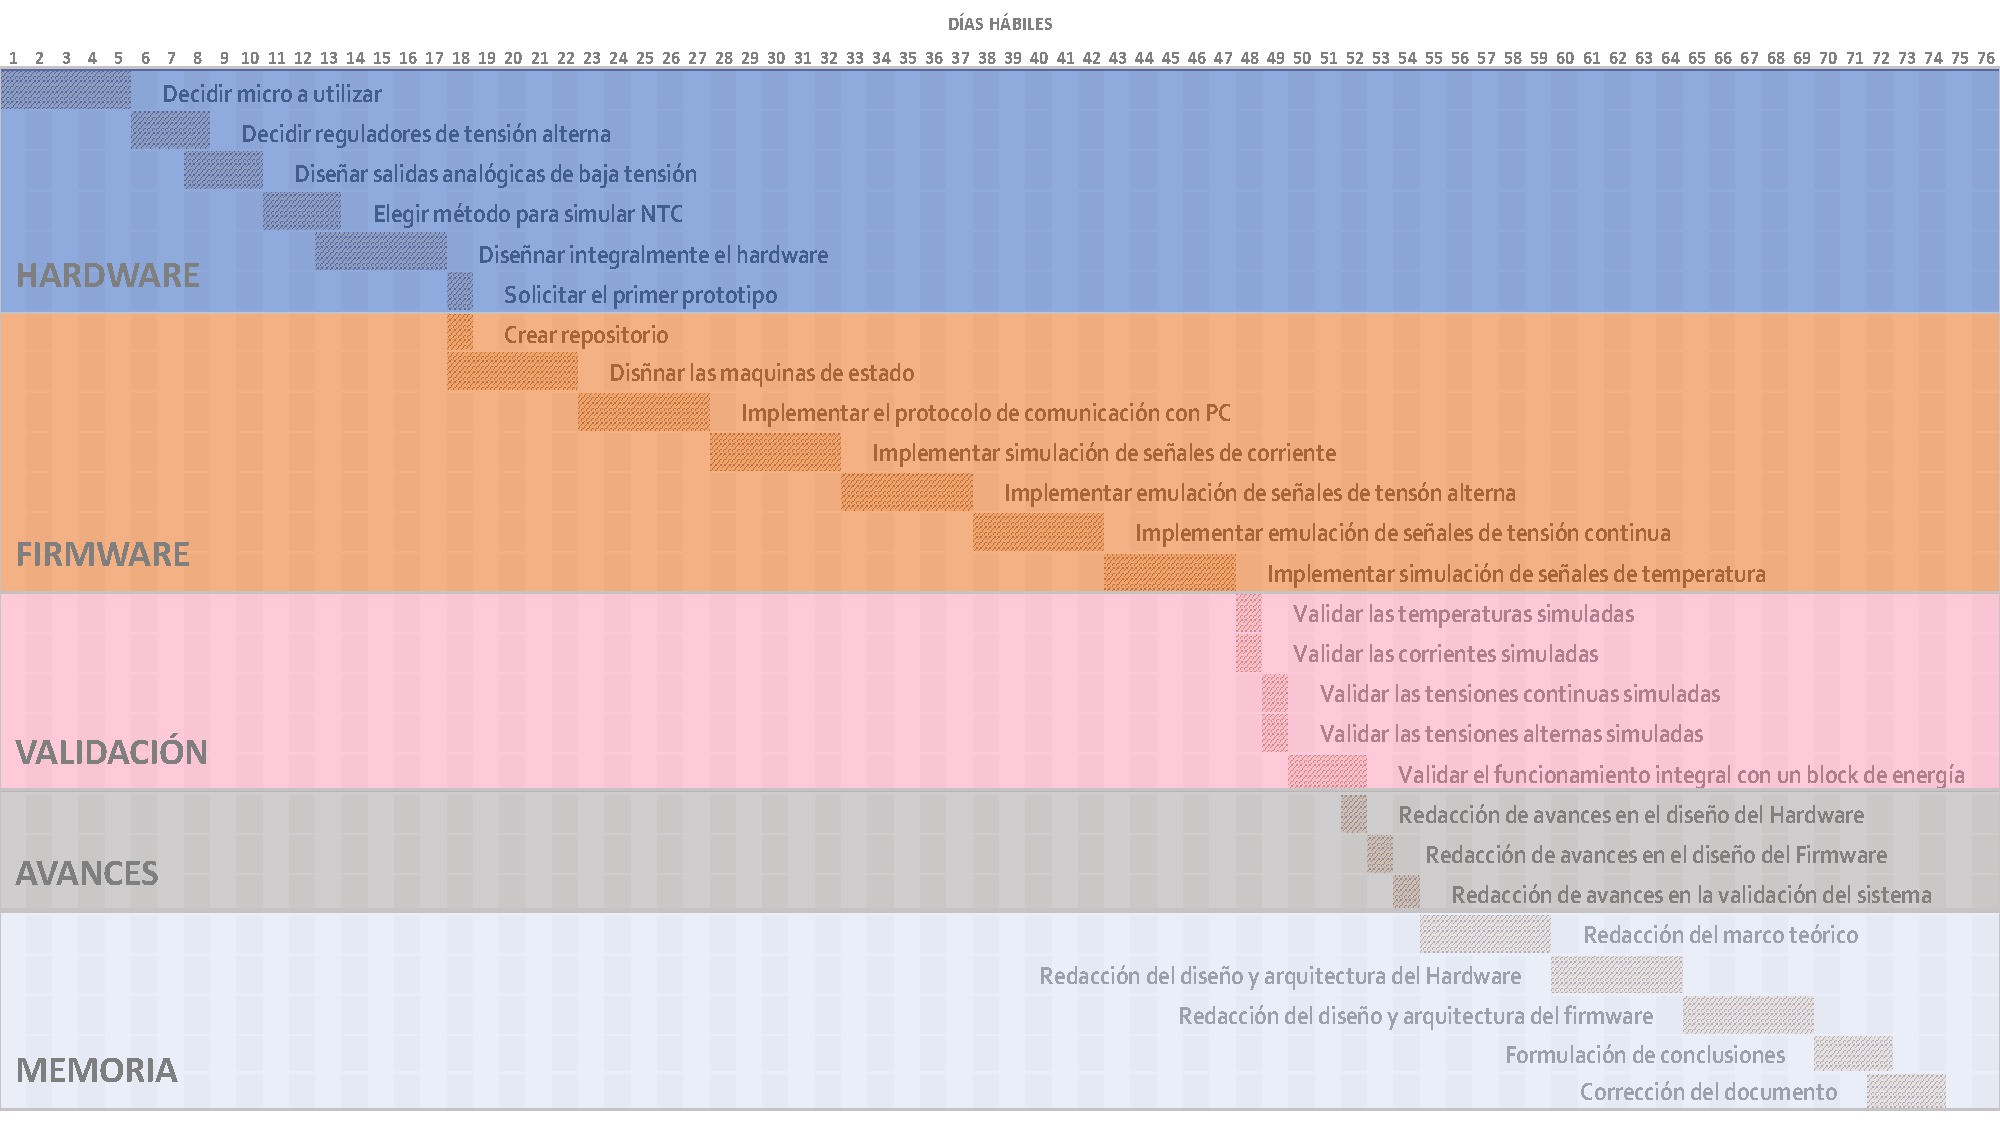
\includegraphics[width=1.5\textheight]{./Figuras/Gantt.pdf}
		\caption{diagrama de Gantt}
		\label{fig:diagGantt}
	\end{figure}

\end{landscape}




\section{12. Presupuesto detallado del proyecto}
\label{sec:presupuesto}

\begin{table}[htpb]
	\centering
	\begin{tabularx}{\linewidth}{@{}|X|c|r|r|@{}}
		\hline
		\rowcolor[HTML]{C0C0C0}
		\multicolumn{4}{|c|}{\cellcolor[HTML]{C0C0C0}COSTOS DIRECTOS}   \\ \hline
		\rowcolor[HTML]{C0C0C0}
		Descripción                                                 &
		\multicolumn{1}{c|}{\cellcolor[HTML]{C0C0C0}Cantidad}       &
		\multicolumn{1}{c|}{\cellcolor[HTML]{C0C0C0}Valor unitario} &
		\multicolumn{1}{c|}{\cellcolor[HTML]{C0C0C0}Valor total}        \\ \hline
		Placa principal                                             &
		\multicolumn{1}{c|}{3}                                      &
		\multicolumn{1}{c|}{10000}                                  &
		\multicolumn{1}{c|}{30000}                                      \\ \hline
		Circuito de potencia                                        &
		\multicolumn{1}{c|}{3}                                      &
		\multicolumn{1}{c|}{15000}                                  &
		\multicolumn{1}{c|}{45000}                                      \\ \hline
		Cableado y componentes de comunicación                      &
		\multicolumn{1}{c|}{3}                                      &
		\multicolumn{1}{c|}{2000}                                   &
		\multicolumn{1}{c|}{6000}                                       \\ \hline
		Honorarios de desarrollador                                 &
		\multicolumn{1}{c|}{600}                                    &
		\multicolumn{1}{c|}{1500}                                   &
		\multicolumn{1}{c|}{900000}                                     \\ \hline
		\multicolumn{3}{|c|}{SUBTOTAL}                              &
		\multicolumn{1}{c|}{981000}                                     \\ \hline
		\rowcolor[HTML]{C0C0C0}
		\multicolumn{4}{|c|}{\cellcolor[HTML]{C0C0C0}COSTOS INDIRECTOS} \\ \hline
		\rowcolor[HTML]{C0C0C0}
		Descripción                                                 &
		\multicolumn{1}{c|}{\cellcolor[HTML]{C0C0C0}Cantidad}       &
		\multicolumn{1}{c|}{\cellcolor[HTML]{C0C0C0}Valor unitario} &
		\multicolumn{1}{c|}{\cellcolor[HTML]{C0C0C0}Valor total}        \\ \hline
		\multicolumn{1}{|l|}{30\% de los costos directos}           &
		\multicolumn{1}{c|}{1}                                      &
		\multicolumn{1}{c|}{294300}                                 &
		\multicolumn{1}{c|}{294300}                                     \\ \hline
		\multicolumn{3}{|c|}{SUBTOTAL}                              &
		\multicolumn{1}{c|}{294300}                                     \\ \hline
		\rowcolor[HTML]{C0C0C0}
		\multicolumn{3}{|c|}{TOTAL}                                 &
		\multicolumn{1}{c|}{1275300}                                    \\ \hline
	\end{tabularx}%
\end{table}


\section{13. Gestión de riesgos}
\label{sec:riesgos}

a) Identificación de los riesgos (al menos cinco) y estimación de sus consecuencias:

Riesgo 1: Demora en la llegada de componentes del exterior.
\begin{itemize}
	\item Severidad (S): 8

	      La demora en la llegada de componentes del exterior, cuando son necesarios, detiene completamente el avance del proyecto.
	\item Probabilidad de ocurrencia (O): 9

	      Las demora de recursos del exterior es muy recurrente en Argentina.
\end{itemize}

Riesgo 2: El vinculo con la empresa se termine en un plazo muy corto.
\begin{itemize}
	\item Severidad (S): 10.

	      No será posible realizar el proyecto.
	\item Ocurrencia (O): 2.

	      El vinculo actual con \clientename\hspace{1px}  es poco probable que finalice debido a que actualmente el autor trabaja en relación de dependencia para el.
\end{itemize}

Riesgo 3: Accidentes graves en las verificaciones del proyecto debido a los riesgos asociados a la alta tensión.
\begin{itemize}
	\item Severidad (S): 10.

	      EL uso de tensiones mayores a 300 V puede causar daños graves y poner en riesgo el avance del proyecto.
	\item Ocurrencia (O): 5.

	      El constante uso de las placas con altas tensiones aumenta el riesgo de que se produzcan accidentes.
\end{itemize}

Riesgo 4: Cancelación del proyecto del block de energía por decisión de la empresa.
\begin{itemize}
	\item Severidad (S): 10.

	      La cancelación del proyecto del block de energía torna innecesario el desarrollo de este proyecto
	\item Ocurrencia (O): 2.

	      La tecnología actualmente es muy demandada y no se presentan amenazas evidentes sobre la continuidad del proyecto.
\end{itemize}

Riesgo 5: Subestimación de tiempos en tareas de la línea crítica
\begin{itemize}
	\item Severidad (S): 6.

	      Este error en la planificación indefectiblemente atrasa todo el plan.

	\item Ocurrencia (O): 7.

	      El poco conocimiento sobre la complejidad del problema a resolver aumenta significativamente las probabilidades de error en la estimación de tiempos.
\end{itemize}
b) Tabla de gestión de riesgos:      (El RPN se calcula como RPN=SxO)
\begin{table}[htpb]
	\centering
	\begin{tabularx}{\linewidth}{@{}|X|c|c|c|c|c|c|@{}}
		\hline
		\rowcolor[HTML]{C0C0C0}
		Riesgo & S  & O & RPN & S* & O* & RPN* \\ \hline
		1      & 8  & 9 & 72  & 8  & 3  & 24   \\ \hline
		2      & 10 & 2 & 20  &    &    &      \\ \hline
		3      & 10 & 5 & 50  & 10 & 1  & 10   \\ \hline
		4      & 10 & 2 & 20  &    &    &      \\ \hline
		5      & 6  & 7 & 42  &    &    &      \\ \hline
	\end{tabularx}%
\end{table}

Criterio adoptado:
Se tomarán medidas de mitigación en los riesgos cuyos números de RPN sean mayores a 45

Nota: los valores marcados con (*) en la tabla corresponden luego de haber aplicado la mitigación.

c) Plan de mitigación de los riesgos que originalmente excedían el RPN máximo establecido:

Riesgo 1: Se definirá con celeridad la lista de componente y se realizara el pedido con anticipación para asegurar un período de tiempo extenso desde que se piden los elementos al exterior hasta que se los necesite.

- Severidad (S): 8

La severidad no varía.

- Probabilidad de ocurrencia (O): 3

La anticipación reduce significativamente la probabilidad de que ocupara.

Riesgo 3: Se utilizará serigrafía en la placa para indicar las regiones de alta tensión, se utilizara las protecciones y aislaciones necesarias para reducir la probabilidad de shock eléctrico.

- Severidad (S): 8

La severidad no varía.

- Probabilidad de ocurrencia (O): 2

La anticipación reduce significativamente la probabilidad de que ocupara.


\section{14. Gestión de la calidad}
\label{sec:calidad}

\begin{enumerate}
	\item Interfases
	      \begin{enumerate}
		      \item El sistema debe poder comunicarse con una PC

		            Verificación: se verifica el envío de las tramas series esperadas para cada comando.

		            Validación: el sistema responde a los comandos seteados por el usuario como espera.
		      \item El sistema debe poseer un botón de encendido

		            Verificación: el sistema enciende al presionar el botón. Las transiciones de tensión son las adecuadas.

		            Validación: el sistema siempre enciende cuando se presiona el botón.

		      \item El sistema debe tener actuadores que simulen una señal de potencia.

		            Verificación: se miden tensiones del 220[V] rms alterna y 450[V] continua en las salidas de potencia al activarlas.

		            Validación: la placa de control detecta las señales de la placa de prueba.
		      \item El sistema debe tener actuadores con señales de baja tensión.

		            Verificación: se miden tensiones del 5[V] continua en las salidas de baja tensión al activarlas.

		            Validación: la placa de control detecta las señales de la placa de prueba.

		      \item El sistema debe tener actuadores resistivos.

		            Verificación: la resistencia varia al setear un cambio. También alcanza los extremos esperados
		            (condicionado por el sensor NTC de la placa de control)

		            Validación: la placa de control mide todo el rango de temperaturas válidas.

		      \item El sistema debe informar el estado de las señales (on/off).
		            Verificación: se observa el encendido de cada LED al activar la señal.

		            Validación: el usuario puede reportar, observando la placa, que señal esta activa en menos de 3 segundos.
	      \end{enumerate}
	\item Requerimientos funcionales
	      \begin{enumerate}
		      \item Emulación de altas tensiones continuas
		            \begin{enumerate}
			            \item El sistema debe controlar salidas de tensión que emulen las tensiones de continua elevadas que mide el block de energía.
			                  Verificación: se miden las tensiones de salida de potencia al activar la señal.

			                  Validación: la placa de control mide las tensiones de continua.
			            \item El sistema debe permitir que el usuario configure el valor de tensión continua elevada a emular.

			                  Verificación: configurando con saltos de 20 V, y en un rango de 0 a 450 V, se miden las tensiones de salida esperadas al activar la señal.

			                  Validación: la placa de control mide las tensiones configuradas de tensión continua.

			            \item El sistema debe reportar error si no se configura un valor válido de tensión.

			                  Verificación: se observa que se reporta un mensaje de error al no configurar un valor válido de tensión. Tampoco se miden las tensiones en la salida de la placa.

			                  Validación: el usuario interpreta el mensaje de error.

			            \item El sistema debe permitir configurar las tensiones elevadas continuas Vbatt, Vbus y Vrelé de la Figura 1 de forma independiente.

			                  Verificación: se verifica que configurando tres valores válidos de Vbatt, Vbus y Vrelé las salidas se miden correctamente. Se debe verificar con 5 V de diferencia entre señales y con 50 V de diferencia entre señales.

			                  Validación: la placa de control mide las tensiones configuradas de tensión.

			            \item El sistema emulará tensiones de bus, batería y relé en un rango comprendido entre 0 V a 450 V.

			                  Verificación: para cada señal se puede verificar que la tensión de salida medida es la configurada en todo el rango de tensiones con saltos de 20 V.

			                  Validación: la placa de prueba mide la misma tensión que la configurada con un error de 5 V.
		            \end{enumerate}
		      \item Simulación de corriente con bajas tensiones de continua
		            \begin{enumerate}
			            \item El sistema debe controlar salidas de tensión que simulen la medición de corriente de los sensores utilizados por el block de energía.
			                  Verificación: se miden las tensiones de salida al activar la señal.

			                  Validación: la placa de control mide corrientes al activar las señales.
			            \item El sistema debe permitir que el usuario configure el valor de corriente a simular.

			                  Verificación: configurando con saltos de 5 A, se miden las tensiones esperadas al activar la señal.

			                  Validación: la placa de control mide las corrientes configuradas de corriente.

			            \item El sistema debe reportar error si no se configura un valor válido de corriente.

			                  Verificación: se observa que se reporta un mensaje de error al no configurar un valor válido de corriente. Tampoco se miden las tensiones en la salida de la placa.

			                  Validación: el usuario interpreta el mensaje de error.
			            \item El sistema debe permitir configurar las corrientes Igrid e Ibatt de la Figura \ref{fig:diagBloques} de forma independiente.

			                  Verificación: se verifica que configurando dos valores válidos de Igrid y Ibatt las salidas se miden correctamente. Se debe verificar con 5 A de diferencia entre señales.
		            \end{enumerate}
		      \item Emulación de tensiones alternas
		            \begin{enumerate}
			            \item El sistema debe controlar salidas de tensión que emulen las tensiones alternas que mide el block de energía.

			                  Verificación: se miden las tensiones de salida al activar la señal.

			                  Validación: la placa de control mide las tensiones alternas.
			            \item El sistema debe permitir que el usuario configure el valor de tensión a emular.

			                  Verificación: configurando con saltos de 20 V, y en un rango de 0 a 240 Vrms, se miden las tensiones de salida esperadas al activar la señal.

			                  Validación: la placa de control mide las tensiones configuradas de tensión.
			            \item El sistema debe reportar error si no se configura un valor válido de tensión alterna.

			                  Verificación: se observa que se reporta un mensaje de error al no configurar un valor válido de tensión alterna. Tampoco se miden las tensiones en la salida de la placa.

			                  Validación: el usuario interpreta el mensaje de error.
			            \item El sistema debe permitir configurar las tensiones alternas Vgrid y Vinverter de la Figura \ref{fig:diagBloques} de forma independiente.

			                  Verificación: se verifica que configurando dos valores válidos de Vgrid y Vinverter las salidas se miden correctamente. Se debe verificar con 5 Vrms de diferencia entre señales y con 50 Vrms de diferencia entre señales.

			            \item El sistema emulará tensiones alternas (Vinverter y Vgrid) en un rango comprendido entre 0 y 240 Vrms.

			                  Verificación: para cada señal se puede verificar que la tensión de salida medida es la configurada en todo el rango de tensiones alternas con saltos de 20 Vrms.

			                  Validación: la placa de prueba mide la misma tensión que la configurada con un error de 5 Vrms.
		            \end{enumerate}
		      \item Simulación de temperaturas
		            \begin{enumerate}
			            \item El sistema debe controlar resistencias variables que emulen la variación de resistencia de un termistor NTC por temperatura.

			                  Verificación: se miden las resistencias de salida al activar la señal.

			                  Validación: la placa de control mide las temperaturas correspondientes a las resistencias de salida.
			            \item El sistema debe permitir que el usuario configure el valor de temperatura a emular.

			                  Verificación: configurando con saltos de 5 C, en un rango de 0 C a 100 C, se miden las resistencias de salida esperadas al activar la señal.

			                  Validación: la placa de control mide las temperaturas configuradas.
			            \item El sistema debe reportar error si no se configura un valor válido de temperatura.

			                  Verificación: se observa que se reporta un mensaje de error al no configurar un valor válido de temperatura. Tampoco se miden las resistencias de salida.

			                  Validación: el usuario interpreta el mensaje de error.
			            \item El sistema debe permitir configurar las temperaturas Tcoil, Tigbt y ambiente de la Figura \ref{fig:diagBloques} de forma independiente.

			                  Verificación: se verifica que configurando dos valores válidos de Tcoil, Tigbt y ambiente las salidas se miden correctamente. Se debe verificar con 5 C de diferencia entre señales.

			                  Validación: la placa de control mide las temperaturas correspondientes a las resistencias de salida.
			            \item El sistema simulará las temperaturas en un rango comprendido entre 5 a 150 ºC.

			                  Verificación: para cada señal se puede verificar que la resistencia de salida medida es la configurada en todo el rango de temperaturas con saltos de 5 ºC.

			                  Validación: la placa de prueba mide la misma resistencia que la configurada con un error de 5 ºC.
		            \end{enumerate}
	      \end{enumerate}
	\item Requerimientos de rendimiento
	      \begin{enumerate}
		      \item El sistema debe actuar en un tiempo menor a 150 ms luego de recibir un comando del usuario.

		            Verificación: se miden los tiempos de respuesta desde que llega la señal por UART a la placa de prueba hasta que se mide una señal a la salida.

		            Validación: el usuario esta conforme con la respuesta del sistema.
	      \end{enumerate}
\end{enumerate}

\section{15. Procesos de cierre}
\label{sec:cierre}

Establecer las pautas de trabajo para realizar una reunión final de evaluación del proyecto, tal que contemple las siguientes actividades:

\begin{itemize}
	\item Pautas de trabajo que se seguirán para analizar si se respetó el Plan de Proyecto original:
	      - Indicar quién se ocupará de hacer esto y cuál será el procedimiento a aplicar.
	\item Identificación de las técnicas y procedimientos útiles e inútiles que se emplearon, y los problemas que surgieron y cómo se solucionaron:
	      - Indicar quién se ocupará de hacer esto y cuál será el procedimiento para dejar registro.
	\item Indicar quién organizará el acto de agradecimiento a todos los interesados, y en especial al equipo de trabajo y colaboradores:
	      - Indicar esto y quién financiará los gastos correspondientes.
\end{itemize}

\begin{itemize}
	\item Análisis de correspondencia con el Plan de Proyecto original.
	      \begin{itemize}
		      \item Responsable: \authorname\hspace{1px}.
		      \item Se analizará cuales fueron los motivos que desviaron a las tareas retrasadas del plan original.
	      \end{itemize}
	\item Identificación de las técnicas y procedimientos útiles e inútiles que se emplearon, y los problemas que surgieron y cómo se solucionaron.
	      \begin{itemize}
		      \item Responsable: \authorname\hspace{1px}.
		      \item Se generará documentación durante el avance del proyecto sobre las técnicas y herramientas recurridas. Al finalizar se realizara un compendio con todas las herramientas que resultaron de mayor utilidad para el desarrollo del proyecto.
	      \end{itemize}
	      \begin{itemize}
		      \item Responsable: \authorname\hspace{1px}.
		      \item Se realizará un acto por la plataforma Meet para agradecer a todos los que hicieron posible el desarrollo del proyecto: colaboradores, profesores de la maestría y el equipo de trabajo.
	      \end{itemize}
\end{itemize}

\end{document}
